%
% Copyright (C) 2011 Agostino De Marco
%                    <agostino dot demarco at unina dot it>
%                    Roberto Giacomelli
%                    <giaconet dot mailbox at gmail dot com>
%
%    This work may be distributed and/or modified under the
%    conditions of the LaTeX Project Public License, either
%    version 1.3 of this license or any later version.
%    The latest version of this license is in
%    http://www.latex-project.org/lppl.txt and version 1.3
%    or later is part of all distributions of LaTeX version
%    2005/12/01 or later.
%
% This work has the LPPL maintenance status `maintained'.
% 
% The Current Maintainer of this work are Agostino De Marco
% and Roberto Giacomelli
%
\documentclass{standalone}
\usepackage{lmodern}
\usepackage{amsmath,fixmath}
\usepackage{relsize}
\usepackage{pgfplots}

\usepgflibrary{decorations.pathmorphing}
\usepgflibrary{shapes.geometric,shapes.misc}

\usepackage{siunitx}
\sisetup{
   load=derived,
   unitsep=thin,
   valuesep=thin,
   decimalsymbol=comma,
   expproduct=cdot,
   digitsep=thin,
   sepfour=false,
   group-digits=false
}
\newunit{\kcal}{kcal}

\pgfplotsset{compat=1.3}

\addtolength{\oddsidemargin}{-5.0cm}

\begin{document}

\pgfkeys{
   /pgf/number format/.cd, 
      %use comma,
      set decimal separator={,{\!}},
      set thousands separator={}
}

\pgfplotsset{
   every axis/.append style={
      font=\relsize{2},
      % very thick,% thick
      % tick style={very thick} % semithick
      line width=1.8pt,% thick
      tick style={line width=1.8pt} % semithick
      },
   every axis x label/.append style={
      font=\relsize{4},
      yshift=0pt,
      xshift=0em
   },
   every axis y label/.append style={
      font=\relsize{3},
      rotate=-90, % -90,
      xshift= 0.8em, % -0.2em,
      yshift=-1.4em, % 0.5em
   },
   major grid style={
      line width = 0.8pt,
      black,
      dash pattern=on 8pt off 4pt
   },
   every axis title/.append style={
      font=\relsize{3}
   }
}

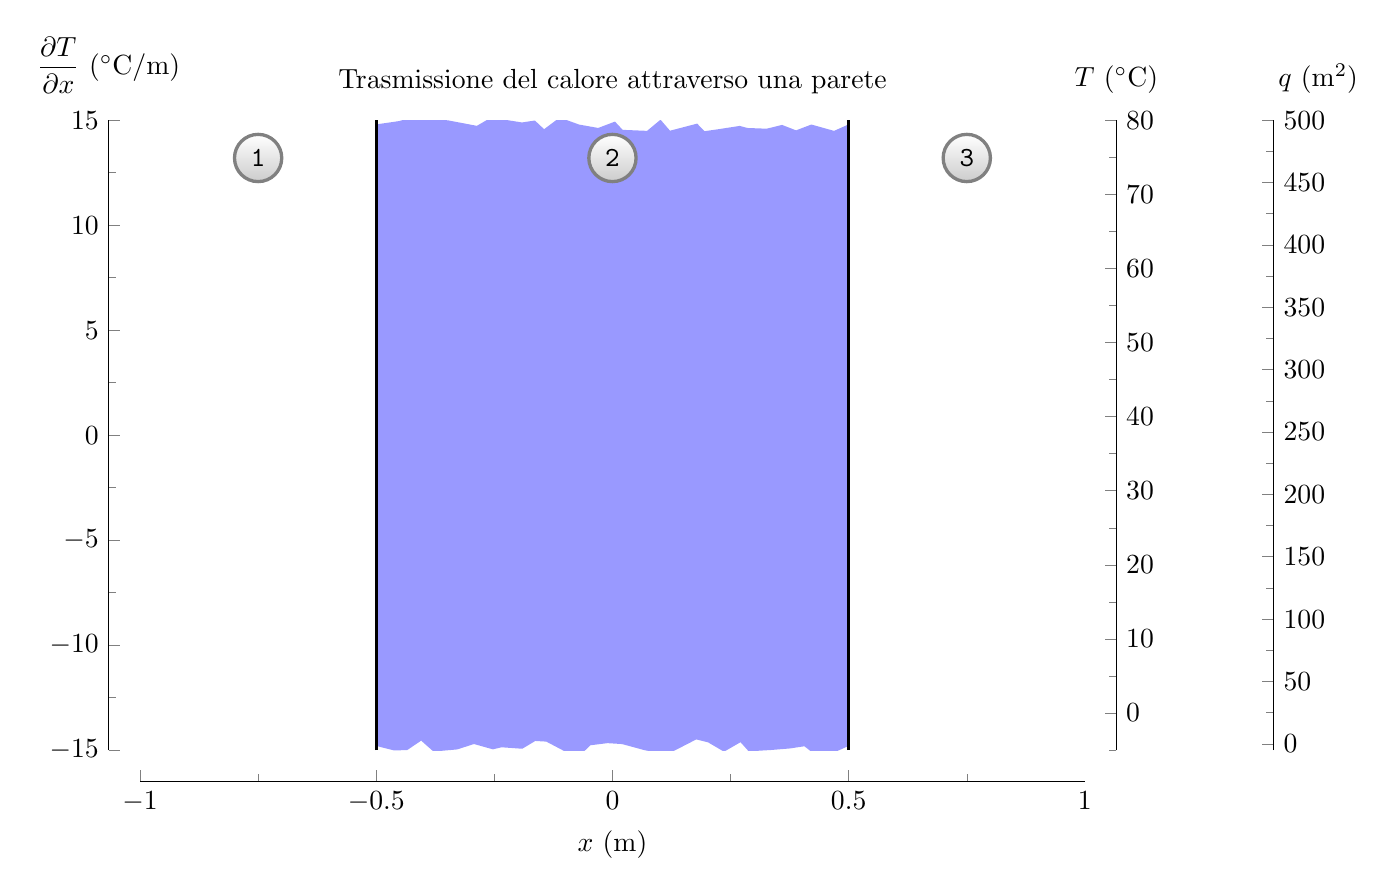
\begin{tikzpicture}
      % provide shared options here with pgfplotsset:
    \pgfplotsset{
        width=12cm,height=8cm,
        no markers
    }

% the left y-axis #1
\begin{axis}[
   clip=false,
   scale only axis,
   width=2cm, xshift=-0.4cm,
   xmin=-1, xmax=1,
   hide x axis,
   axis y line*=left,% the '*' avoids arrow heads
   ymin=-15, ymax=15,
   ytick={-15,-10,...,15},
   minor y tick num = 1,
%   ylabel={
%      \parbox{2cm}{%
%               \centering
%               $\dfrac{\partial T}{\partial x}$
%               \\[0.7em]
%               \centering
%               (\si{\celsius/\meter})
%      }
%   },
]
\node [above, yshift=6pt] at (rel axis cs:0,1) {$\dfrac{\partial T}{\partial x}$ (\si{\celsius/\meter})};
\end{axis}

% the unique x-axis
\begin{axis}[
   scale only axis,
   height=2cm, yshift=-0.4cm,
   xmin=-1, xmax=1,
   xtick={-1,-0.5,...,1},
   minor x tick num = 1,
   xlabel={$x$ (\si{\meter})},
   axis x line*=bottom,% the '*' avoids arrow heads
   hide y axis,
   ymin=-15, ymax=15,
]
\end{axis}

% the curve #1
\begin{axis}[
   scale only axis,
   xmin=-1, xmax=1,
   hide x axis,
   ymin=-15, ymax=15,
   hide y axis,
   title=\parbox{8cm}{\centering Trasmissione del calore attraverso una parete},
]
\fill[blue!40]
    %[decoration={random steps,segment length=2mm},decorate,very thick] 
    decorate [decoration={random steps,segment length=2mm}] { [very thick] (axis cs:-0.5,-14.8) -- (axis cs:0.5,-14.8) }
    -- (axis cs:0.5,14.8)
    decorate [decoration={random steps,segment length=2mm}] { [very thick] -- (axis cs:-0.5,14.8)}
    -- cycle;
\draw[very thick] (axis cs:-0.5,-15) -- (axis cs:-0.5,15);
\draw[very thick] (axis cs:0.5,-15) -- (axis cs:0.5,15);

\node [rounded rectangle, minimum size=6mm, very thick, draw=black!50, top color=white, bottom color=black!20, font=\ttfamily]
   at (rel axis cs:0.125,0.94) {1};
\node [rounded rectangle, minimum size=6mm, very thick, draw=black!50, top color=white, bottom color=black!20, font=\ttfamily]
   at (rel axis cs:0.50,0.94) {2};
\node [rounded rectangle, minimum size=6mm, very thick, draw=black!50, top color=white, bottom color=black!20, font=\ttfamily]
   at (rel axis cs:0.875,0.94) {3};
\end{axis}

\pgfplotsset{
   every axis y label/.append style={
      xshift= -2.4em
   }
}

% the right y-axis 2
\begin{axis}[
   clip=false,
   scale only axis,
   xshift=0.4cm,
   xmin=-1, xmax=1,
   hide x axis,
   axis y line*=right,% the '*' avoids arrow heads
   ymin=-5, ymax=80,
   ytick={-10,0,...,80},
   minor y tick num = 1,
%   ylabel={
%      \parbox{2cm}{%
%               \centering
%               $T$
%               \\[0.0em]
%               \centering
%               (\si{\celsius})
%      }
%   },
]
\node [above, yshift=6pt] at (rel axis cs:1,1) {$T$ (\si{\celsius})};
\end{axis}

\pgfplotsset{every axis y label/.append style={xshift=-1.3em}}

% the right y-axis 2
\begin{axis}[
   clip=false,
   scale only axis,
   xshift=2.4cm,
   xmin=-1, xmax=1,
   axis x line=none,
   hide x axis,
   axis y line*=right,% the '*' avoids arrow heads
   ymin=-5, ymax=500,
   ytick={0,50,...,500},
   minor y tick num = 1,
%   ylabel={
%      \parbox{4cm}{%
%               \centering
%               $T^4-T_0^4$
%               \\[0.0em]
%               \centering
%               (\si{\celsius^4})
%      }
%   },
]
\node [above, yshift=6pt, xshift=16pt] at (rel axis cs:1,1) {$q$ (\si{\kcal/\meter^2})};
\end{axis}

\end{tikzpicture}


\end{document}